%
% File coling2014.tex
%
% Contact: jwagner@computing.dcu.ie
%%
%% Based on the style files for ACL-2014, which were, in turn,
%% Based on the style files for ACL-2013, which were, in turn,
%% Based on the style files for ACL-2012, which were, in turn,
%% based on the style files for ACL-2011, which were, in turn, 
%% based on the style files for ACL-2010, which were, in turn, 
%% based on the style files for ACL-IJCNLP-2009, which were, in turn,
%% based on the style files for EACL-2009 and IJCNLP-2008...

%% Based on the style files for EACL 2006 by 
%%e.agirre@ehu.es or Sergi.Balari@uab.es
%% and that of ACL 08 by Joakim Nivre and Noah Smith

\documentclass[11pt]{article}
\usepackage{coling2014}
\usepackage{times}
\usepackage{url}
\usepackage{latexsym}
\usepackage{hyperref}
\usepackage{todonotes}
\usepackage{textcomp}
\usepackage{graphicx}
\graphicspath{ {images/} }
%\setlength\titlebox{5cm}

% You can expand the titlebox if you need extra space
% to show all the authors. Please do not make the titlebox
% smaller than 5cm (the original size); we will check this
% in the camera-ready version and ask you to change it back.

\newcommand{\TODO}[1]{\todo[inline]{{\footnotesize #1}}}

\title{An Overview over \\ Autonomous Vehicles}

\date{}

\begin{document}
\maketitle
\begin{abstract}
\TODO{Abstract}
\end{abstract}

\section{Introduction}
Soon traversing the streets of Gothenburg the future of \textit{Autonomous Vehicles} (AV) is coming closer to being a part of today's reality. The dream of self driving cars holds many promises, with one of it's bigger points being safety.

In 2011 more than 2.2 million injuries were caused by automobile crashes in the United States alone \cite[p. 14]{Anderson2014rand}, while more than 39 percent of all fatalities involved alcohol \cite[p. 16]{Anderson2014rand}. With a far greater field of vision, reaction time and control of safety-critical functions, the hopes is that AV could drastically reduce these statistics.

With efficient and aware driving as well as the possibilities of higher space efficiency self driving cars could vastly reduce fuel consumption and CO$_2$ emissions \cite[p. 28ff]{Anderson2014rand} meanwhile increasing the convenience, reliability and personal independence of those not capable of driving themselves \cite[p. 17]{Anderson2014rand}.

Throughout history man has tried to create a self driving car using very different technologies. As early as 1926 a driverless car drove the streets of Milwaukee. At the time the car had to be radio-controlled from a following car \cite{Sentinel1926Phantom}. In the following decades many companies tried to add various sensors in the roads. They were able sense the presence of any vehicle and would send information to that vehicles autopilot \cite{Courier1960Driverless}.

A big step towards technology of today was the DARPA Grand Challenge, launched by the Defence Advance Research Projects Agency (DARPA) in 2003. The challenge was to develop an AV that could pass a 142-mile course of unrehearsed off-road terrain. The first race held in 2004 was completed without finishing vehicles, and in race 2005 the robot Stanley would become the first vehicle to finish the race.

While Stanley was designed for a static environment and would be unable to travel on populated roads it shares many similarities to technologies of the AVs today. It used a combination of GPS and several sensor, such as RADAR mounted on the roof, to get an accurate position and used laser terrain mapping to identify obstacles on the path. Combined with advanced software this meant it could map an area of 200m ahead and could react to obstacles. Today this technology has advanced to the point it can recognize pedestrians and other traffic \cite{Thrun2006stanley}.

AVs faces both ethical and legal question, such as who is responsible in the event of an accident or where to crash in the case it's unavoidable. Despite this most believe in a future of AVs, the majority of car companies are today researching AVs and in early 2014 Induct started selling Navia, the first commercial self driving car \cite{Maisto2014Navia}.


\section{How AVs work}
\subsection{Sensors}
In order for the autonomous vehicles to navigate the real world, its software needs to obtain data about itself and its surroundings. For that purpose, AVs have several types of sensors incorporated to its body. The software processes the data provided by those sensors to create a virtual representation of the real world which can then use to calculate which actions to take to reach its destination. There are two main types of sensors: Exterioceptive and proprioceptive. The former deals with information from the AV's environment, while the later deals with information internal to the system. Some examples of the data that can be obtained within each class are:
\begin{itemize}
	\item Extereoceptive: Distances to objects, object types, objects' speed and heading.
	\item Proprioceptive: Motor speed, wheel load, heading, position, battery status.
\end{itemize}
For a more functional perspective, the sensors can be organized into categories defined by its use cases for AVs:
\begin{itemize}
	\item \textbf{Know where you are going}:
		\begin{itemize}
			\item \textbf{GPS}: It allows the AV to determine its position in absolute terms. In optimal conditions it has good accuracy and precision. It cannot be constantly relied upon due to intermittent coverage caused by tunnels, canyons, buildings, radio interference, etc. \cite{SchweberMouser}
			\item \textbf{IMU} (Inertial Measurement Unit): A type of dead-reckoning\footnote{Dead-reckoning is the process of calculating one's current position by using a previously determined position, and advancing that position based upon known speeds over elapsed time and course.} system using a 3-axis accelerometer providing data on linear motion, and a 3-axis gyroscope providing data on rotational motion. This data is then used to calculate the motion and relative position of the vehicle regardless of any sort of signal obstruction. It has good accuracy for short periods but has cumulative error so over time it gets very inaccurate.
			\item \textbf{Compass}: It can be used to determine the AV's heading. It has good accuracy which doesn't change over time but it is subject to interference by magnetic objects and electrical sources. It also can be slow to settle except for the most expensive types.
			\item \textbf{Ground speed RADAR}: Measures real ground speed using the Doppler effect. It can be used for dead-reckoning.
			\item \textbf{Wheel odometry}: Used for dead-reckoning. Uses optical encoders to measure the speed of the wheels and the direction of the steering wheel from which the relative position of the AV can be calculated.
		\end{itemize}
	\item \textbf{See where you are going}:
		\begin{itemize}
			\item \textbf{LIDAR}: The device emits laser pulses, and measures the time the beam takes to reflect back to the sensor (Time-of-flight), then it calculates the distance using that measurement. By using a rotating, scanning mirror assembly on top of the AV, it provides 3D 360{\textdegree} view suitable for ``big picture'' imaging. It is not very effective for close-in control.
			\item \textbf{Cameras}: They are typically used to enhance the resolution of the 3D information obtained by the LIDAR, as well as detecting street signs and road markings. Its effectiveness is affected by reduced visibility conditions such as dusk, bad weather and dirt on the lens.
			\item \textbf{RADAR}: Similar to LIDAR but instead of laser it uses a normal radio wave beam (usually 77GHz) to measure distance. It is used for close-in control instead of LIDAR: Parking, lane-changing and bumper-to-bumper traffic.
		\end{itemize}
	\item \textbf{Get where you are going}:
		Other sensors are needed for the correct operation of the AV, which deal with the internal state of the vehicle, such as: Battery \& fuel level sensors, engine temperature, oil pressure, etc.
\end{itemize}

\subsection{Software}
\TODO{``figure out'' might be too colloquial?}
\TODO{it's not clear that we're talking about Google cars only. Where to mention that?}
In order to use the sensors to actually drive humans need to program how to interpret all the data the sensors collect. The main concerns of AV are driving, and avoiding all other objects. The cars use the sensors to figure out where they are. Google has created very specific maps for the cars to use to find there location. These maps include everything about an area including curb height, intersection width, and lane layout. 
The cars figure out where they are by matching the images from the sensors to
a specific place on the map. They use where the car was a few seconds prior to help them make location matches in real
time. The preinstalled maps are not a perfect solution. For example the
cars are not able to drive in snow because the snow changes the landscape and therefore the physical markers google
usually uses to place a car. While the cars rely on the maps immensely it knows that roads do change. They are
constantly sending data back to google about changes in roads because of erosion or construction. 


After the cars figure out exactly where they are they need to then worry about cars, pedestrians, and cyclists.
Within those categories there is more specific categorizations. For example the cars differinatiate between, trucks or
road worker in orange vests. They also look out for common things in the road like traffic cones. Once they recognize
that there is something the computers use machine learning techniques to
differentiate between every possibility. Once the car guesses what type of object it is it starts to make assumptions
about what the object will do next. If a car is driving straight it assumes the car will continue to drive straight. If
a car is in the turning lane it will probably turn. The cars are programmed to anticipate the next move while also
keeping in mind that might not happen. If the car sees something in the road that is cannot recognize it stops. 


Because these cars are programmed to there choices are very automatic. It is relativity easy to predict how they will act
exactly how people have programmed them. While they are far from perfect Google has gone very far to make them at least as
reliable as human drivers. Google has an entire team dedicated to testing. 
\begin{figure}[!ht]
  \centering
      \reflectbox{%
                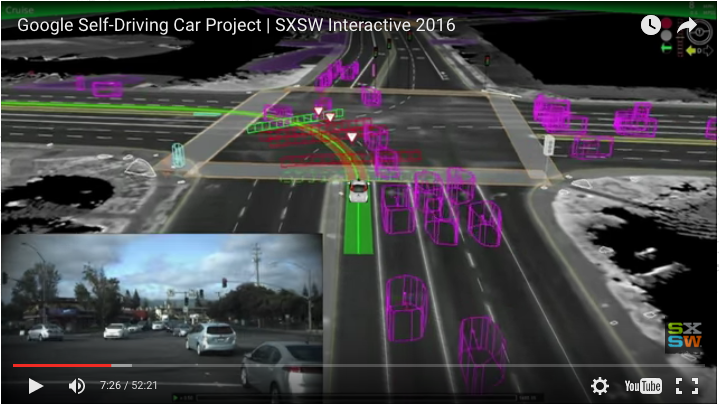
\includegraphics[width=0.7\textwidth]{drivingcar}}
                  \caption{The small box to the right is a picture from the front window of the car. The rest of the
                      image is how the car interprets images from the sensors. The purple boxes are other motored
                          vehicles. The blue box on the crosswalk is a person. The green track is where the car has to
                          go. The long green and red cylinders and the projected motion of cars that would end up in the
                  path of the car.}
\end{figure}


\section{Social and Ethical Implications of AVs}
\subsection{Impact on society in general}
The introduction of autonomous vehicles could drastically decrease the individual cost of transportation, especially because the passenger can use the transportation time for work or other activities. According to Anderson et al. this will most likely lead to ``low-density patterns of land-use surrounding metropolitan regions'' \cite{Anderson2014rand}, because longer distances to the workplace will be acceptable.

The overall effect on energy consumption and emissions is unclear: on the one hand, the total vehicle miles traveled might increase due to reduced opportunity cost for time spent in the car. On the other hand, the technology also offers various possibilities to decrease emissions, including light-weight vehicles and platooning.

AVs could bring independence and mitigated social isolation for those unwilling or unable to drive. Note however that for this to actually make a difference society has to ensure that all members of society can actually profit from the new technology.

\subsection{Economics}
Many jobs and a variety of professions will likely be affected by the introduction of AVs. In 2015, roughly 1.18 million bus and truck drivers have been employed in the US according to the Bureau of Labor Statistics \cite{USLabourBureau2016}, and those are only two examples of professions which would obviously be affected in a very direct way. Decreasing crash risks could impair the business of many insurance companies, and since AVs could facilitate the introduction of alternative fuels, jobs related to combustion engines might become obsolete. According to Anderson et al. ``... lost jobs might be replaced by others, perhaps related to the AV industry, but there may be considerable economic disruption'' \cite[p. 40ff]{Anderson2014rand}. Not only technical solutions necessary here, but also appropriate policy reactions and extensive discussion and changes in society. The impact of automization on the labour market and possible policy reactions, including a basic income, are currently being discussed controversially \cite{VanDerVeen2002, Olsen2014}.

AVs will, just like most state-of-the-art technology, likely be very expensive in the first years. Thus, this presumably safe, fast, reliable and convenient mean of transportation might be only available to the richer parts of the population. Driving conventional cars could become a necessity for the poor, further increasing the social gap between rich and poor \cite[p. 39]{Anderson2014rand}.

\subsection{Liability}
The AV manufacturer's liability will likely increase, which according to Anderson et al. ``could lead to inefficient delays in adoption of this technology''. Amongst others companies, Volvo has stated that it accepts full liability for accidents caused by their AV technology \cite{HarrisVolvo2015}. Manufacturers could try to mitigate the risks involved in accident liability by providing vehicles as a service instead of as a product. In any case, states will have to establish legal frameworks for autonomous driving. 
\TODO{mention: federal insurance backstop, or simply assign liability to human drivers? \textit{tort preemption??}}

\subsection{Ethical Decision Making}
In a study on ethical decision making during AV crashes, Goodall came to the conclusion that $(1)$ AVs would almost certainly crash, $(2)$ that an AV's decisions that preceded certain crashes have a moral component, and that $(3)$ there is no obvious way to encode complex human morals effectively in software \cite{Goodall2014ethical}. Current approaches to AV ethics can be divided into two groups: rational and \textit{AI} (Artifical Intelligence) approaches. 

In the former, an AV must either adhere to a predefined set of rules or try to minimize some clearly defined function, which usually represents the total damage to humans, environment and property. These approaches are easy to implement and tailor-made for execution by computers, but the incompleteness of any set of rules and the difficulty involved in the articulation of complex human ethics as a set of rules are problematic. No matter how many rules are fed into such a system, there will always be situations in which the resulting behaviour does not match the expectations of human ethics.

The basic idea of \textit{Artificial Intelligence} (AI) approaches to AV ethics is to train a \textit{neural network} (NN) on a combination of simulations and recordings of real crashes, with human feedback on the ethical response. This solves the problem of having to encode the complex human ethics into a mathematical set of rules. However, the inconsistency between how humans actually behave and what they believe, and lacking traceability (why did the NN decide the way it did in an accident?) involve a risk of missing transparency and manipulation. NNs capable of providing natural-language feedback of how they came to certain decisions are a active field of resear+ch \cite[p. 63]{Goodall2014ethical}. 

Goodall proposes a three-phase ethical vehicle deployment strategy \cite[p.63]{Goodall2014ethical} which can be compared to the moral education of a child. In the first phase, rational ethics are used, i.e. the AV must follow some clearly defined rules. In the second phase, a hybrid rational and AI approach is used: The strict rules from phase one remain active as a boundary, but additionally the complex specifics of human ethics are learned using AI technology. In the third phase, once the technical obstacles have been overcome, natural language feedback should be added to the AI technology of phase two. Current state-of-the-art AVs are in the first of these three phases. \TODO{add citation, and I assume that there's at least active research happening right now for the other two proposed phases?!}

\section{Conclusion}
\TODO{Conclusion}
\subsection{Future of AVs}
...
\subsection{Our Predictions}



\TODO{Gerd: I created a BibTex bibliography file (Bibliography.bib), and added the bibtex code for some of our references. Now this has to be done for the other references as well. I moved the old bibliography code to OldBibliography.tex until we've entirely switched to bibtex. You can usually find the complete BibTex code for most books and articles by simply googling the title + ``bibtex'' or by using google scholar and pressing the ``cite'' button there.}

% BibTeX 
\bibliographystyle{IEEEtran}
%\bibliographystyle{acl}
%\bibliography{acl2014}
\bibliography{Bibliography}


\end{document}

%%% Local Variables:
%%% mode: latex
%%% TeX-master: t
%%% End:
